%************************************************
\chapter{Application development}\label{ch:application-overview}
%************************************************

\section{Requirements specification}

\hiddensubsection{Generation of mock data}
As described in \autoref{sec:problem-description}, we want to develop an application which can translate natural language questions that refers to entities in a database or index owned by a software development company. This project has been made with strong collaboration with Findwise, a company with focus on search driven solutions. Findwise has an index with information about employees, projects and customers, however, it is not possible to use their information because it is confidential and cannot be published in a master thesis. A different approach to get hold of relevant data is to generate mock data that is inspired by Findwise's data model. Mock data in this project is simply generated data from files that can be used to simulate a real world example application.

\hiddensubsection{Grammar development}\label{sec:grammar-development}
The grammar in \autoref{ch:simple-grammar} can only translate the instruction \texttt{people who know Java} in English and Swedish into Solr query language. The grammar needs to be extended to handle \emph{any} programming language that exists in the mock data, not only \texttt{Java}. The grammar also needs to support more instructions in order to make a more realistic use case. We have chosen the to support the following instructions:

\begin{figure}[H]
\begin{terminal}
English                        Solr query language
people who know Java           q= object_type : Person AND KNOWS : Java
people who work in London      q= object_type : Person AND WORKS_IN : London
people who work with Unicef    q= object_type : Person AND WORKS_WITH : Unicef
customers who use Solr         q= object_type : Customer AND USES : Solr
projects who use Solr          q= object_type : Project AND USES : Solr
\end{terminal}
\caption{All sentences supported by the application\label{fig:suppported-sentences}}
\end{figure}

Two more cases has been added to instructions regarding \emph{people}. In addition, two new type of instructions has been added, translations about \emph{customers} and \emph{projects}. Note that \autoref{fig:suppported-sentences} only shows specific instances of instructions. These instances are based on data in the mock-database, where we assume that the words \emph{Java}, \emph{London}, \emph{Unicef} and \emph{Solr} exists in the database. It should be possible to express every word available in the database in an instruction. For example if \emph{Paris} is a city in the database we can create the instruction \emph{people who work in Paris}.

\hiddensubsection{Suggestions}\label{sec:suggestions}
If a user has no idea of which instructions the application can translate, how can she use the application? This thesis uses a narrow application grammar, which means that it only covers specified sentences. Therefore, if a sentence has one character in the wrong place, GF will not be able to
translate anything. This problem can be solved by using a wide coverage grammar, an example of an application that adopts this technique is the GF android app \cite[p. 41]{angelov2014speech}. This project, however, does not.

GF has the power to suggest valid words of an incomplete sentence by using incremental parsing \cite{angelov09:incremental-parser}. This means that even though a user do not know what to type, the application can suggest valid words to use. If the user chooses to add one of those words, the suggestion engine can show a new list of words that will match the new partial sentence.

However, this method does not support the use of only keywords, since one cannot start a sentence with for example the word \texttt{Java}. It it also inflexible since it does not support the use of words outside the grammar, e.g. \texttt{all people who know Java}\marginpar{The parser would not be able to parse the word \emph{all}}.

This thesis takes a different approach on a suggestion engine. Instead of suggesting one word at a time, one can suggest a whole sentence based on what the user has typed so far. This is achieved by generating all possible sentences that the application can translate and indexing them in Apache Solr. This makes it very easy to search on matching sentences, we also gain powerful techniques such as approximate string matching. 
\newline
\newline
By using this approach, if a user types a sentence in the application, it will search in the index on instructions related to the string and retrieve the most relevant instructions.

As the suggestion engine uses a search platform, it is possible to type anything and get suggestions, even only keywords like \texttt{'people java'} will suggest instructions that can be formulated with these two words.

\hiddensubsection{Runtime environment}
The chosen programming language for this project is Java. The main reason is because it is Findwise's primary programming language. It is also very well known among many companies in the world.
Many professional Java-developers adopts a specific development platform, Java Enterprise Edition (Java EE). This platform provides many libraries that can be scaled to work in an enterprise environment. This project also adopts Java EE.

\hiddensubsection{Handling dependencies}
A typical Java EE project make use of several libraries, in computer science terms we say that a project can have other libraries as \emph{dependencies}. It is not unusual that these libraries also have their own dependencies. Larger projects can therefore have a lot of dependencies, so many that it becomes hard to keep track of them. This project make use of an open source tool called Apache Maven to handle dependencies. One simply list all libraries the project shall have access to, then Maven will automatically fetch them and their dependencies. This also makes the application more flexible, as it do not have to include the needed libraries in the application.

\hiddensubsection{Input and output presentation}
Besides handling translation and suggestions, the application also needs to handle input and present its results in some way. This application takes input and presents output by using a web gui\footnote{\url{http://en.wikipedia.org/wiki/Graphical_user_interface}}.

To summarize, this application is a web application built in Java EE and uses Apache Maven for library management.

\hiddensubsection{Running the application}
Web applications built in Java are usually has the WAR file format. It is a special JAR-file which includes classes, dependencies and web pages. This project uses an open source web server called Apache Tomcat to host a web application by exporting our application as a WAR-file. Apache Tomcat will make the application available by using HTTP-requests and spawn a new thread for each request.
\newline
\newline
Details about the runtime environment can be found in \autoref{ch:appendix-a} and \autoref{ch:appendix-b}.

\section{Grammar development with the RGL}
This section continues the work on the grammar introduced in \autoref{ch:simple-grammar}.

\hiddensubsection{Supported instructions}
The example grammar could only translate one instruction. This instruction in English is \emph{people who know Java}. It is easy to extend this grammar to support more programming languages, for example, to support \emph{Python} one can add a function \texttt{Python : Object} in the abstract syntax and implement it as \texttt{Python = "python"} in the concrete syntaxes. However, this approach makes the grammar inflexible because we need to extend the grammar every time we want to add a new programming language.

\hiddensubsection{Names}
Defining a new function for each programming language is not a good idea, it forces us to update the grammar every time we want it to support a new programming language. A better solution would be to make one function that could be used by any programming language.

One intuitive approach to solve this problem is to create a function \texttt{MkObject : String -> Object}. The implementation for this function would be 
\begin{figure}[H]
\begin{code}
-- Abstract syntax
MkObject : String -> Object ;
-- RGL implementation
MkObject str = mkNP (mkPN str.s) ; -- PN = Proper Name
-- Solr implementation
MkObject str = str.s ;
\end{code}
\caption{Intuitive approach on names}
\end{figure}

The GF-code compiles, and the parsing and linearization by using Solr query language works. Unfortunately, this approach does not work with the RGL. GF cannot create a proper name by using an arbitrary string. \todo{Why?}

Fortunately, there exists a built in category which can be used for exactly these situations. We use the category \texttt{Symb}, along with the function \texttt{MkSymb : String -> Symb} to represent arbitrary strings. We can then use the function \texttt{SymbPN} to create a proper name and finally create a noun phrase.
\begin{figure}[H]
\begin{code}
-- Abstract syntax
MkObject : Symb -> Object ;
-- RGL implementation
MkObject symb = mkNP (SymbPN symb) ; -- PN = Proper Name
-- Solr implementation
MkObject symb = symb.s ; -- Symb has the type { s : Str }
\end{code}
\caption{Working approach on names}
\end{figure}

By using this solution, we can translate the sentence \emph{people who know foo}, where \emph{foo} can be anything.

\hiddensubsection{Extending the grammar}
It is not trivial to extend the grammar to support the instructions described in \autoref{sec:grammar-development}. One has to take into account that it shall not be possible to translate invalid instructions like \emph{projects who work in London}. We will in this section first extend the abstract syntax to support the new instructions and then extend the concrete syntaxes.

\subsubsection*{Abstract syntax}

The first step towards a solution to this problem is to modify the abstract syntax. We begin by removing the category \texttt{Subject} and replacing it with three new categories: \texttt{Internal}, \texttt{External} and \texttt{Resource}. The function \texttt{People} will return a value of the type \texttt{Internal} and \texttt{Customer} and \texttt{Project} will return values of the types \texttt{External} and \texttt{Resource} respectively.

\begin{figure}[H]
\begin{code}
-- Instructions.gf
cat
  Internal ;
  External ;
  Resource ;
fun
  People   : Internal ;
  Customer : External ;
  Project  : Resource ;
\end{code}
\caption{Abstract syntax with new categories and functions for subjects}
\end{figure}

In addition to adding new subject categories, three new categories for relations are also introduced: \texttt{InternalRelation}, \texttt{ExternalRelation} and \texttt{ResourceRelation} (\texttt{Relation} is removed). The idea is to link subject values to the correct relation types. For instance, we link a value of the type \texttt{Internal} with a value of type \texttt{InternalRelation}.

All relation functions are changed to return the correct type. For example, \texttt{Know} is changed to return a value of the type \texttt{InternalRelation}. This means that only \texttt{People} can be used together with \texttt{Know}, as desired. The new relation implementations can be seen in \autoref{fig:newrelations}.

\begin{figure}[H]
\begin{code}
cat
  InternalRelation ;
  ExternalRelation ;
  ResourceRelation ;
fun
  Know     : Object -> InternalRelation ;
  UseExt   : Object -> ExternalRelation ;
  UseRes   : Object -> ResourceRelation ;
  WorkIn   : Object -> InternalRelation ;
  WorkWith : Object -> InternalRelation ;
\end{code}
\caption{Abstract syntax with new categories and functions for relations \label{fig:newrelations}}
\end{figure}

The last thing to modify is how subjects and relations are combined. The function \texttt{MkInstruction} is replaced by three new functions: \texttt{InstrucInternal}, \texttt{InstrucExternal} and \texttt{InstrucResource}. However, as we do not need to make any distinction between different type of instructions at this level, all three functions returns a value of the type \texttt{Instruction}.

\begin{figure}[H]
\begin{code}
cat
  Instruction ;
fun
  InstrucInternal : Internal -> InternalRelation -> Instruction ;
  InstrucExternal : External -> ExternalRelation -> Instruction ;
  InstrucResource : Resource -> ResourceRelation -> Instruction ;
\end{code}
\caption{Abstract syntax with new categories and functions for instructions\label{fig:newinstructions}}
\end{figure}

\hiddensubsubsection{Concrete syntax using the RGL}
As the abstract syntax has changed, the concrete syntaxes has to be modifed as well. This section explains how the generalised concrete syntax which uses the RGL is implemeneted. 

\autoref{fig:rgl-new-categories} shows how the categories has been implemented. The new categories are implemented in the same way as the previous.

\begin{figure}[H]
\begin{code}
lincat
  Instruction = NP ;
  Internal, External, Resource = N ;
  InternalRelation, ExternalRelation, ResourceRelation = VP ;
\end{code}
\caption{Concrete syntax using the RGL with new category implementations\label{fig:rgl-new-categories}}
\end{figure}

The new subject functions are implemented in the same way as \texttt{People}.

\begin{figure}[H]
\begin{code}
lin
  People = person_N ;
  Customer = customer_N ;
  Project = project_N ;
\end{code}
\caption{RGL concrete syntax with new subject implementations\label{fig:rgl-new-subjects}}
\end{figure}

Four new relation functions are added. Line 5-6 in \autoref{fig:rgl-new-relations} shows how we use the verb \texttt{work\_V} together with two prepositions, \texttt{in\_Prep} and \texttt{with\_Prep} in order correctly linearize into \emph{work in foo} and \emph{work with foo} respectively (\emph{foo} is the value of \texttt{object}. The relation implementations make use of an operation \texttt{mkRS'} to reuse code.

\begin{figure}[H]
\begin{code}
lin
  Know object = mkRS' (mkVP know_V2 object) ;
  UseExt object = mkRS' (mkVP use_V2 object) ;
  UseRes object = mkRS' (mkVP use_V2 object) ;
  WorkIn object = mkRS' (mkVP (mkV2 work_V in_Prep) object) ;
  WorkWith object = mkRS' (mkVP (mkV2 work_V with_Prep) object) ;

oper
  -- Make a relative sentence
  mkRS' : VP -> RS = \vp -> mkRS (mkRCl which_RP vp) ;
\end{code}
\caption{Concrete syntax using the RGL with new relation implementations\label{fig:rgl-new-relations}}
\end{figure}

Subjects and relations are combined as before, but as this solution has three functions instead of one, a new operation \texttt{mkQ} has been defined in order to reuse code.

\begin{figure}[H]
\begin{code}
lin
  InstrucInternal internal relation = mkI internal relation ;
  InstrucExternal external relation = mkI external relation ;
  InstrucResource resource' relation = mkI resource' relation ;

oper
  mkI : N -> RS -> NP = \noun,rs -> mkNP aPl_Det 
                             (mkCN noun rs) ;
\end{code}
\caption{Concrete syntax using the RGL with new instruction implementations\label{fig:rgl-new-instructions}}
\end{figure}

\subsubsection*{Concrete syntax for Solr}
This section describes how the concrete syntax for Solr is modified to work with the new abstract syntax.

The new categories are all defined as strings.

\begin{figure}[H]
\begin{code}
lincat
  Instruction = Str ;
  Internal, External, Resource = Str ;
  InternalRelation, ExternalRelation, ResourceRelation = Str ;
  Object = Str ;
\end{code}
\caption{Solr concrete syntax with new implementation of categories\label{fig:solr-categories-impl}}
\end{figure}

Subject types are hard coded into strings. We assume that these strings exists in the Solr index.

\begin{figure}[H]
\begin{code}
lin
  People = "Person" ;
  Customer = "Organization" ;
  Project = "Project" ;
\end{code}
\caption{Solr concrete syntax with new subject implementations\label{fig:solr-function-implementation}}
\end{figure}

We also make an assumption about how the relations are defined in the Solr index. 

\begin{figure}[H]
\begin{code}
lin
  Know obj = "KNOWS" ++ ":" ++ obj ;
  UseExt obj = "USES" ++ ":" ++ obj ;
  UseRes obj = "USES" ++ ":" ++ obj ;
  WorkWith obj = "WORKS_WITH" ++ ":" ++ obj ;
  WorkIn obj = "WORKS_IN" ++ ":" ++ obj ;
\end{code}
\caption{Solr concrete syntax with new relation implementations\label{fig:solr-new-relations}}
\end{figure}

As in the concrete syntax using the RGL, also an operation is defined and used by the three functions.

\begin{figure}[H]
\begin{code}
lin
  InstrucInternal internal relation = select internal relation ;
  InstrucExternal external relation = select external relation;
  InstrucResource resource' relation = select resource' relation;

oper
  select : Str -> Str -> Str = \subj,relation -> 
                    "select?q=*:*&wt=json&fq=" ++ "object_type :" 
                    ++ subj ++ "AND" ++ relation ;
\end{code}
\caption{Solr concrete syntax with new instruction implementations\label{fig:solr-new-instructions}}
\end{figure}

\hiddensubsection{Boolean operators}
The grammar is now powerful enough to translate a variety of questions. To make it even more powerful, one could use boolean operators in order to combine relations. For example, an instruction that could be useful is \emph{people who know Java and Python}. Another useful instruction is \emph{people who know Java and work in Gothenburg}. This section explains how the grammar can be extended to support these kind of instructions.

In addition to the previous example with the boolean operator \emph{and}, we will also add support for the boolean operator \emph{or}. We begin by adding functionality to support boolean operators to combine values of the type \texttt{Object}. As seen in \autoref{fig:boolean-abs-obj}, two new functions are defined in the abstract syntax to handle these cases, one for each operator.

\begin{figure}[H]
\begin{code}
lin
  And_O : Object -> Object -> Object ;
  Or_O : Object -> Object -> Object ;
\end{code}
\caption{Abstract syntax for boolean operators and objects\label{fig:boolean-abs-obj}}
\end{figure}

The RGL implementation is shown in \autoref{fig:boolean-rgl-obj}.

\begin{figure}[H]
\begin{code}
lin
  And_O o1 o2 = mkNP and_Conj o1 o2 ;
  Or_O o1 o2 = mkNP or_Conj o1 o2 ;
\end{code}
\caption{Concrete syntax using the RGL for boolean operators and objects\label{fig:boolean-rgl-obj}}
\end{figure}

The Solr implementation is shown in \autoref{fig:boolean-solr-obj}. We add \texttt{AND} or \texttt{OR} between the two objects.

\begin{figure}[H]
\begin{code}
lin
  And_O o1 o2 = "(" ++ o1 ++ "AND" ++ o2 ++ ")" ;
  Or_O o1 o2 = "(" ++ o1 ++ "OR" ++ o2 ++ ")" ;
\end{code}
\caption{Solr concrete syntax for boolean operators and objects\label{fig:boolean-solr-obj}}
\end{figure}

It is now possible to express \emph{people who know Java and Python}. In order to use boolean operators with whole relations like \emph{people who know Java and work in Gothenburg}, the grammar has to be further extended.

We must also take into account that it shall only be possible to combine relationship that are possible to express in the current sentence. Therefore, we need to define the boolean logic three times, as we have three different types of instructions.

\begin{figure}[H]
\begin{code}
lin
  InternalAnd : InternalRelation -> InternalRelation -> InternalRelation ;
  InternalOr : InternalRelation -> InternalRelation -> InternalRelation ;

  ExternalAnd : ExternalRelation -> ExternalRelation -> ExternalRelation ;
  ExternalOr : ExternalRelation -> ExternalRelation -> ExternalRelation ;
 	  
  ResourceAnd : ResourceRelation -> ResourceRelation -> ResourceRelation ;
  ResourceOr : ResourceRelation -> ResourceRelation -> ResourceRelation ;
\end{code}
\caption{Abstract syntax for boolean operators and relations\label{fig:boolean-abstract-relations}}
\end{figure}

Instead of combining noun phrases as in \autoref{fig:boolean-rgl-obj}, here we combine relative sentences in the RGL implementation.

\begin{figure}[H]
\begin{code}
lin
  InternalAnd rs1 rs2 = mkRS and_Conj rs1 rs2 ;
  InternalOr rs1 rs2 = mkRS or_Conj rs1 rs2 ;
	  
  ExternalAnd rs1 rs2 = mkRS and_Conj rs1 rs2 ;
  ExternalAnd rs1 rs2 = mkRS or_Conj rs1 rs2 ;
	  
  ResourceAnd rs1 rs2 = mkRS and_Conj rs1 rs2 ;
  ResourceOr rs1 rs2 = mkRS or_Conj rs1 rs2 ;
\end{code}
\caption{Concrete syntax using the RGL for boolean operators and relations\label{fig:boolean-rgl-relations}}
\end{figure}

The Solr implementation is fairly straight forward, similarly as with values of the type \texttt{Object}, we also add \texttt{AND} or \texttt{OR} between the strings. The only difference is that we do it three times as we have three different subject types.

\begin{figure}[H]
\begin{code}
lin
  InternalAnd s1 s2 = "(" ++ s1 ++ "AND" ++ s2 ++ ")";
  InternalOr s1 s2 = "(" ++ s1 ++ " OR " ++ s2 ++ ")";

  ExternalAnd s1 s2 = "(" ++ s1 ++ "AND" ++ s2 ++ ")";
  ExternalOr s1 s2 = "(" ++ s1 ++ " OR " ++ s2 ++ ")";

  ResourceAnd s1 s2 = "(" ++ s1 ++ "AND" ++ s2 ++ ")";
  ResourceOr s1 s2 = "(" ++ s1 ++ " OR " ++ s2 ++ ")";
\end{code}
\caption{Solr concrete syntax for boolean operators and relations\label{fig:boolean-solr-relations}}
\end{figure}

\section{Suggestion engine}
This section continues where \autoref{sec:suggestions} left off. The suggestion engine shall generate all possible instructions in all natural languages and store them in an Apache Solr index. It is suitable to use the \emph{generator} which GF creates to generate abstract syntax trees and linearize them into the specified concrete languages (English and Swedish in this case).

The generator can be accessed through the GF-shell.  \autoref{fig:gf-shell-generate-trees} shows how the function \texttt{generate\_trees} is executed to generate all trees with the \emph{depth} 4. By depth, we mean the maximum number edges between a leaf and the root element.

\begin{figure}[H]
\begin{terminal}
Instrucs> generate_trees
InstrucExternal Customer (UseExt (MkObject (MkSymb "Foo")))
InstrucInternal People (Know (MkObject (MkSymb "Foo")))
InstrucInternal People (WorkIn (MkObject (MkSymb "Foo")))
InstrucInternal People (WorkWith (MkObject (MkSymb "Foo")))
InstrucResource Project (UseRes (MkObject (MkSymb "Foo")))
\end{terminal}
\caption{\texttt{generate\_trees} is used to create all abstract syntax trees with max depth 4\label{fig:gf-shell-generate-trees}}
\end{figure}

\autoref{fig:gf-shell-generate-trees} shows 5 trees, but there exists many more trees.\marginpar{Actually, there exists infinitely many trees, as we have recursive functions in the abstract syntax.} The reason GF only generates 5 trees is because of the default depth setting is 4. If we increase the depth we will obtain more trees, as it then will include trees containing boolean operators. By increasing the max depth to 5, GF will generate 36 trees. With depth 6, GF will generate 321 trees.
\newline
\newline
It is often good to visualize trees to understand them better. \autoref{fig:asts-depths} shows two abstract syntax trees, the first one with depth 4 and the second with depth 5. One can easily see that the former has maximum 4 edges between root and leaf, and the latter has maximum 5 edges between root and leaf.

\begin{figure}[H]
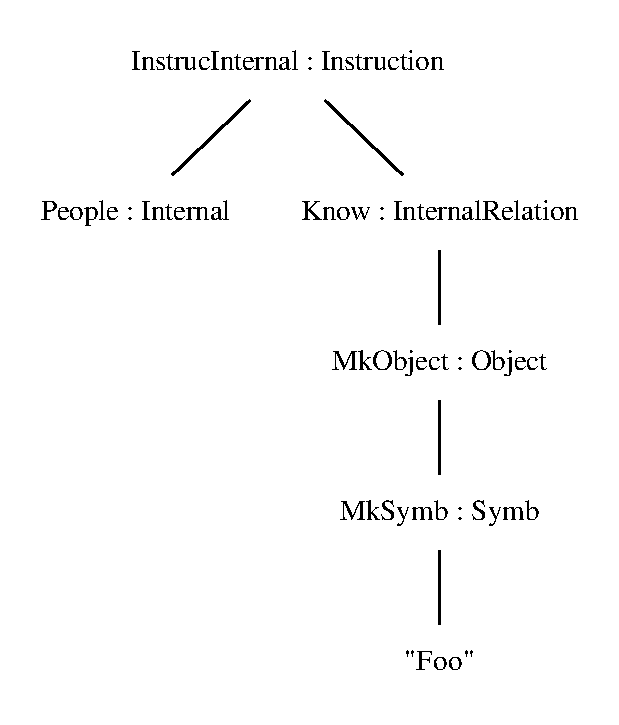
\includegraphics[scale=0.6,keepaspectratio,valign=t]{./gfx/depth4}
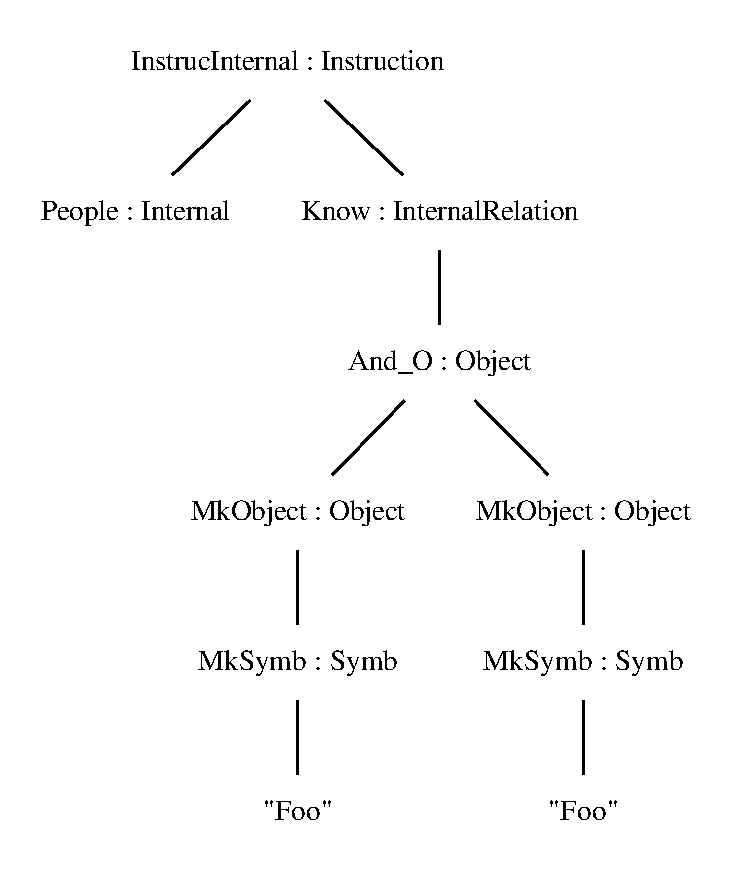
\includegraphics[scale=0.6,keepaspectratio,valign=t]{./gfx/depth5}
\caption{Visualization of abstract syntax trees with depth 4 and 5\label{fig:asts-depths}}
\end{figure}

\hiddensubsection{Populating the Solr index}
It is now time to linearize the generated trees and store them in a Solr index that is dedicated to store linearizations. By doing so, we will be able to search on instructions by using words that exists in the instructions. What we cannot do is to search on names, because the names does not occur in the instructions, instead they only contain a placeholder for a name (\emph{"Foo"}). It will therefore only suggest instructions like \emph{people who know Foo and Foo} which is a useless suggestion.

We want to be able to suggest relevant names. If the user database contains a person which knows Java, then we also want to suggest instructions based on that name. This requirement forces us to change the application once more. 
\newline
\newline
A na{\"i}ve solution would be to fetch all distinct names from the database and create all possible instructions that a user shall be able to express with these names. For an instruction like \emph{people who know Foo or Foo and works in Foo} and if the database contains 10 programming languages and 5 cities we would then have to generate $10*10*5=500$ instructions. This is clearly not suitable, as GF generates 321 trees (with depth 6).
\newline
\newline
A better approach on the problem is to store all distinct names in a separate index. When a user begins to type an instruction, the application checks each word the user has typed. If a word exists in the name-index, then treat it as a name and replace it with \texttt{Foo}, then query the linearizations index. Retrieve the results, and change back \texttt{Foo} to the original name. However, as the application do not make any distinction between different type of names, we could end up with suggestions like \emph{people who work in Python}, because \emph{Python} was replaced by \emph{Foo}. Luckily, this problem can be resolved by introducing a distinction between different types of names in the grammar.

\hiddensubsection{Introducing name types}

This application uses four different kind of names. Programming languages are used together with the \texttt{Know} relation. Organizations are used with the \texttt{Work\_With} relation. Locations are used with the \texttt{Work\_In} relation. Lastly, modules are used with the \texttt{Use} relation. We extend the grammar to support these new name types.

\autoref{fig:abstract-syntax-name-types} shows the new abstract syntax. Line 3 defines new name types. Line 7-10 defines how the names are instantiated. Lines 13-23 defines how names can be combined by using boolean operators. Note how we use the type \texttt{Skill} for programming languages.

\begin{figure}[H]
\begin{code}
cat
  -- Names
  Skill ; Organization ; Location ; Module ;
  
fun
  -- Create unknown names
  MkSkill : Symb -> Skill ;
  MkOrganization : Symb -> Organization ;
  MkModule: Symb -> Module ;
  MkLocation : Symb -> Location ;
  
  -- Boolean operators for Organizations
  And_S : Skill -> Skill -> Skill ;
  Or_S : Skill -> Skill -> Skill ;

  And_O : Organization -> Organization -> Organization ;
  Or_O : Organization -> Organization -> Organization ;

  And_L : Location -> Location -> Location ;
  Or_L : Location -> Location -> Location ;

  And_M : Module -> Module -> Module ;
  Or_M : Module -> Module -> Module ;
\end{code}
\caption{Abstract syntax with new name types\label{fig:abstract-syntax-name-types}}
\end{figure}

The concrete syntax for these new functions are implemented in the same way as the ones we removed (category \texttt{Object} and functions \texttt{MkObject}, \texttt{And\_O} and \texttt{Or\_O}). We have omitted the new concrete syntaxes from the thesis as they do not contribute to anything new.
\newline
\newline
As the grammar has changed, also the abstract syntax trees has changed. \autoref{fig:new-trees-different-types} shows how GF now generate all trees with depth 4.
\begin{figure}[H]
\begin{terminal}
Instrucs> generate_trees
InstrucExternal Customer (UseExt (MkModule (MkSymb "Foo")))
InstrucInternal People (Know (MkSkill (MkSymb "Foo")))
InstrucInternal People (WorkIn (MkLocation (MkSymb "Foo")))
InstrucInternal People (WorkWith (MkOrganization (MkSymb "Foo")))
InstrucResource Project (UseRes (MkModule (MkSymb "Foo")))

\end{terminal}
\caption{Abstract syntax trees with name types\label{fig:new-trees-different-types}}
\end{figure}

As the index stores the linearizations of each tree it is important to post process each linearization in order to preserve the type information. Currently, the type of each name would be lost when linearized, for example \texttt{MkSkill (MkSymb "Foo")} is linearized into just \texttt{"Foo"} if using the english concrete syntax.

To preserve type information, we replace each \texttt{"Foo"} with the current name type $+$ an index. \autoref{fig:preserve-types-example} shows an example.

\begin{figure}[H]
\begin{terminal}
InstrucInternal People (InternalAnd (Know 
            (And_S (MkSkill (MkSymb "Skill0")) (MkSkill (MkSymb "Skill1")))) 
            (WorkIn (MkLocation (MkSymb "Location0"))))
\end{terminal}
\caption{An abstract syntax tree with name types and changed names\label{fig:preserve-types-example}}
\end{figure}

The previous example linearizes into \emph{people who know Skill$0$ and Skill$1$ and who work in Location$0$} by using the concrete syntax for English. We generate all trees again, linearize them into all natural languages and store them in the linearizations index.

In addition, as we store each name in a separate index, we associate each name with its type. By doing so, we can easily find out if a word is a name and then find out what type that name has. 
%By doing so, when we find out if a word the user has typed is a name, we can also find out what type that name is. We then replace the name with its type and add an index that we keep track of in the application. The resulting string can be used to query the linearizations index, as it no longer contains any information about a specific name, it only contains the name type. The result from the linearizations index is a list of suggestions. We change back the type to the original word and present the result to the user.
\newline
\newline
The grammar and the Solr indices are now complete. The application can now suggest relevant sentences even though the user only has typed names (provided that the names exists in the name index).  \autoref{fig:psuedocode-suggestions} shows the pseudocode for the suggestion algorithm with informative comments. This algorithm is executed by the Java-application when a user has typed a partial question.

\begin{figure}[H]
\begin{java-code}
suggestions(sentence) {
    // sentence = "persons who knew java or python and work in London"
    // names[] = {Java, Python, London}
    names[] = extractNames(sentence);
    
    // "persons who knew java or python and work in London" ===> 
    // "persons who knew Skill0 or Skill1 and work in Location0"
    sentence = replaceNamesWithTypes(sentence, names);
    
    // suggestions =
    //   { "people who know Skill0 or Skill1 and who work in Location0", ... }
    suggestions[] = findSentences(sentence);
    
    foreach suggestion in suggestions {
        // "people who know Skill0 or Skill1 and who work in Location0" ===> 
        // "people who know Java or Python and who work in London"
        suggestion = restoreNames(names, suggestion);
    } 
    return suggestions; 
}
\end{java-code}
\caption{Pseudocode for the suggestion algorithm\label{fig:psuedocode-suggestions}}
\end{figure}

\hiddensubsubsection{Supporting invalid sentences}
This section aims to add better accuracy of the suggestion engine by linearizing different variations of a sentence. While the linearization function in GF returns a string representation of a tree, there also exists a parameter \texttt{-list} which allows GF to return all semantically equivalent ways of expressing a sentence.

\begin{figure}[H]
\begin{terminal}
Languages: InstrucsEng
Instrucs> p "people who know Java" | l -list
people who know Java, people's who know Java
\end{terminal}
\caption{Linearization to InstrucsEng using \texttt{-list}\label{fig:linearize-using-list}}
\end{figure}
\todo{Here we actually get four results, three duplicates! Fix, but how?}

\autoref{fig:linearize-using-list} shows that \texttt{people who know Java} actually can be expressed in two ways. We add both linearizations as a list to the same object in the linearizations index, and we list the one we think is the most suitable in the beginning of the list. This makes it possible to search for everything the grammar can parse, but get a more suitable suggestion. For instance, if type \emph{people's who know Java} then the application will match the lesser suitable sentence in the index, but return \emph{people who know Java} as a suggestion.
\newline
\newline
It is possible to add more linearizations than those listed in \autoref{fig:linearize-using-list}. GF adopts the pipe symbol to express that two elements are semantically equivalent. The following sections describes how the pipe symbol can be used to further extend the grammar.

We extend the grammar to treat a subject in singular form the same as a subject in plural form. I.e. the sentences \emph{a person which knows Java} is the same as \emph{people who know Java}. As we treat them equivalent, they will have the same abstract syntax tree, and this tree will linearize to only one Solr query, hence if we translate \emph{a person who knows Java} into Solr, we will obtain a query that retrieves multiple results. The implementation of this extension is achieved by modifying the operation \texttt{mkI}. The reason why the plural version is chosen as the preferable sentence is because \texttt{aPl\_Det} is listed before \texttt{aSg\_Det}.

\begin{figure}[H]
\begin{code}
oper
  mkI : N -> RS -> NP = \noun_N,rs_RS -> mkNP (aPl_Det | aSg_Det)
                             (mkCN noun_N rs_RS) ;
\end{code}
\caption{Treating singular form equivalent to plural form\label{fig:linearize-using-list}}
\end{figure}

The second extension is to treat the \emph{progressive form} of a verb as the same as the regular form. A progressive form of a verb indicates that something is happening right now or was happening or will be happening. The grammar in this project only supports present tense, so it will only cover progressive verbs which expresses that something is happening right now. This is achieved by using the variance function again.

\begin{figure}[H]
\begin{code}
oper
  mkRS' : VP -> RS = \vp -> mkRS (mkRCl which_RP (vp | progressiveVP vp)) ;
\end{code}
\caption{Treating progressive verb equivalent normal form\label{fig:linearize-using-list}}
\end{figure}

However, not all verbs can be used in progressive form. An example of such verb is \emph{know}. An example of  \emph{know} in progressive form is \emph{people who are knowing Java} which clearly is incorrect. Although it might look ugly, it is not an issue for our application as the suggestion engine only suggest the most suitable suggestion. The extension will contribute to make the suggestion engine richer as it allows users to use incorrect instructions.

\section{Alternative implementation without the RGL}\label{sec:english-concat}
We have implemented the concrete syntax for English by using the RGL. This section shows how the same functionality can be achieved by concatenating strings. The purpose of this section is to be able to compare the complexity of a concrete syntax developed by using RGL and by concatenating strings.\newline
\newline
As we concatenate strings in this implementation, all categories are defined as strings.

\begin{figure}[H]
\begin{code}
lincat
 Instruction = Str ;
 Internal, External, Resource = Str ;
 InternalRelation, ExternalRelation, ResourceRelation = Str ;
 Skill, Organization, Location, Module = Str ;
\end{code}
\caption{Concrete syntax for English by concatenating strings with implementation of categories\label{fig:concat-english-cat}}
\end{figure}

In order to achieve the same functionality as the concrete syntax using the RGL, we use variance of strings to support both singular and plural forms. We also use variance to make \emph{persons} a synonym for \emph{people}.

\begin{figure}[H]
\begin{code}
lin
 People = "people" | "persons" | "person" ;
 Customer = "customers" | "customer" ;
 Project = "projects" | "project" ;
\end{code}
\caption{Concrete syntax for English by concatenating strings with implementation of subjects\label{fig:concat-english-subjects}}
\end{figure}

As with subjects, variance is also used with relations.

\begin{figure}[H]
\begin{code}
lin
 Know_R obj = ("know" | "knows") ++ obj;
 UseExt_R obj = ("use" | "uses") ++ obj ;
 UseRes_R obj = ("use" | "uses") ++ obj ;
 WorkWith_R obj = ("work with" | "works with") ++ obj ;
 WorkIn_R obj = ("work in" | "works in") ++ obj ;
\end{code}
\caption{Concrete syntax for English by concatenating strings with implementation of relations\label{fig:concat-english-relations}}
\end{figure}

An instruction is created by concatenating a subject with a relation. In between them we use variance to support connecting words \emph{who, which} and \emph{that}.

\begin{figure}[H]
\begin{code}
lin
 InstrucInternal internal relation = internal ++ 
                                  ("who" | "which" | "that") ++ relation ;
 InstrucExternal external relation = external ++ 
                                  ("who" | "which" | "that") ++ relation ;
 InstrucResource resource' relation = resource' ++ 
                                  ("which" | "that") ++ relation ;
\end{code}
\caption{Concrete syntax for English by concatenating strings with implementation of instructions\label{fig:concat-english-instrucs}}
\end{figure}

A name is just a string.

\begin{figure}[H]
\begin{code}
lin
 MkSkill s = s.s ;
 MkOrganization s = s.s ;
 MkLocation s = s.s ;
 MkModule s = s.s ;
\end{code}
\caption{Concrete syntax for English by concatenating strings with implementation of name\label{fig:concat-english-names}}
\end{figure}

Two names are combined by adding the boolean operator in between them.

\begin{figure}[H]
\begin{code}
lin
 And_S s1 s2 = s1 ++ "and" ++ s2 ;
 Or_S s1 s2 = s1 ++ "or" ++ s2 ;
	  
 And_O s1 s2 = s1 ++ "and" ++ s2 ;
 Or_O s1 s2 = s1 ++ "or" ++ s2 ;
	  
 And_L s1 s2 = s1 ++ "and" ++ s2 ;
 Or_L s1 s2 = s1 ++ "or" ++ s2 ;
	  
 And_M s1 s2 = s1 ++ "and" ++ s2 ;
 Or_M s1 s2 = s1 ++ "or" ++ s2 ;
\end{code}
\caption{Concrete syntax for English by concatenating strings with implementation of boolean operators for names\label{fig:concat-english-boolean-names}}
\end{figure}

As with boolean operators for names, two relations are combined by adding the boolean operator in between them.

\begin{figure}[H]
\begin{code}
lin
 InternalAnd s1 s2 = s1 ++ "and" ++ s2 ;
 InternalOr s1 s2 = s1 ++ "or" ++ s2 ;

 ExternalAnd s1 s2 = s1 ++ "and" ++ s2 ;
 ExternalOr s1 s2 = s1 ++ "or" ++ s2 ;

 ResourceAnd s1 s2 = s1 ++ "and" ++ s2 ;
 ResourceOr s1 s2 = s1 ++ "or" ++ s2 ; 
\end{code}
\caption{Concrete syntax for English by concatenating strings with implementation of boolean operators for relations\label{fig:concat-english-boolean-relations}}
\end{figure}

\section{Generation of mock data}
This section describes how the data used by the application is generated. In order to generate data, we must know what to generate. From \autoref{sec:grammar-development} we know the Solr queries our index must support. We have three different types of objects: \emph{Customer}, \emph{Person} and \emph{Project}. Each of these types of objects has their own data. A customer shall have one value, a list of technologies it uses. A person shall have three values, a list of programming languages it knows, a list of cities it works in and a list of organizations it has been working with. A project shall have one value, the same as a customer, a list of technologies it uses. In addition to these requirements by the grammar, customers and persons also have names. \autoref{fig:example-data-json} shows an example of data that could exists in the Solr index.

\begin{figure}[H]
\begin{js-code}
{ // Customer
  "name" : "Amnesty"
  "object_type" : "Customer",
  "USES" : ["Solr", "Tomcat", "GF"]
},
{ // Person
  "name" : "Jane Doe"
  "object_type" : "Person",
  "KNOWS" : ["Java", "Python", "C"],
  "WORKS_IN" : ["London", "Gothenburg"],
  "WORKS_WITH" :  ["Amnesty", "Unicef"]
},
{ // Project
  "object_type" : "Project",
  "USES" : ["Android", "GF"]
}
\end{js-code}
\caption{Example data in JSON\label{fig:example-data-json}}
\end{figure}

Mock data is generated by combining data from text-files. We have two text-files concerning personal names (\texttt{first\_names.txt} and \texttt{last\_names.txt}). One text-file with organization names (\texttt{charity\_organizations.txt}). One text file about programming languages (\texttt{programming\_languages.txt}). Lastly, one text file containing cities (\texttt{cities.txt}). 

An object is generated by taking one value from each text file that the object needs. For instance, to create an object of the type \texttt{Person}, we fetch values from \texttt{first\_names.txt}, \texttt{last\_names.txt}, \texttt{programming\_languages.txt}, \texttt{cities.txt} and \texttt{charity\_organizations.txt}. The object is then exported to Solr to be stored in the index.